\subsubsection*{Parton level comparisons}

We start the comparison of the various predictions by a comparison at the level of the cross section.
The fiducial volume is the one described in Eqs.~\eqref{cut:1}-\eqref{cut:4}.
The results are documented in Tables~\ref{table:xsectLOfix} and \ref{table:xsectLOdyn}.
There, the cross sections for both processes ${\rm p} {\rm p} \to {\rm e}^+  \nu_{\rm e}  \mu^+ \mu^- {\rm j} {\rm j}$ and ${\rm p} {\rm p} \to {\rm e}^-  \bar \nu_{\rm e}  \mu^+ \mu^- {\rm j} {\rm j}$ at fixed and dynamical scales are presented.
The predictions are clearly not in statistical agreement but they usually agree within about one per cent apart from {\sc MG5\_aMC}.
For the later, the difference can probably be attributed to a miss configuration of the run.
In general, too aggressive estimations of the statistical errors as well as miss-configurations of the run cannot be excluded.

\begin{table}
\begin{center} 
\begin{tabular}{ c | c | c }
 $\mu = \mu_{\rm fix}$ / $\sigma_{\rm LO}^{\rm EW}$ [fb] & ${\rm p} {\rm p} \to {\rm e}^+  \nu_{\rm e}  \mu^+ \mu^- {\rm j} {\rm j}$  & ${\rm p} {\rm p} \to {\rm e}^-  \bar \nu_{\rm e}  \mu^+ \mu^- {\rm j} {\rm j}$  \\
  \hline\hline
  {\sc MG5\_aMC}                  & $0.2783(3)$     & $0.1615(2)$   \\
  {\sc MoCaNLO}+{\sc Recola}      & $0.28496(6)$    & $0.16718(3)$  \\
  {\sc Sherpa}                    & $0.2885(2)$     & $0.1670(2)$   \\
  {\sc VBFNLO}                    & $0.2867(5)$     & $0.1661(3)$   \\
  \hline
\end{tabular}
\end{center}
\caption{
\KL{There is a consistent bias low in my MG numbers. Since it is clearly correlated with low mjj/etajj, any idea what cut might be behaving differently?}
Fiducial cross sections at LO for the process ${\rm p}{\rm p}\to{\rm e}^+\nu_{\rm e}\mu^+\mu^-{\rm j}{\rm j}$ and ${\rm p}{\rm p}\to{\rm e}^-\bar\nu_{\rm e}\mu^+\mu^-{\rm j}{\rm j}$ at order $\mathcal{O} (\alpha^6)$.
The predictions are expressed in fb and are for the LHC running at a centre-of-mass energy of $\sqrt{s}=13 {\rm~TeV}$.
The scale used in the simulations is $\mu = \mu_{\rm fix} = M_W$.
The integration errors of the last digits are given in parentheses.}
\label{table:xsectLOfix}
\end{table}

\begin{table}
\begin{center} 
\begin{tabular}{ c | c | c }
 $\mu = \mu_{\rm dyn}$ / $\sigma_{\rm LO}^{\rm EW}$ [fb] & ${\rm p} {\rm p} \to {\rm e}^+  \nu_{\rm e}  \mu^+ \mu^- {\rm j} {\rm j}$  & ${\rm p} {\rm p} \to {\rm e}^-  \bar \nu_{\rm e}  \mu^+ \mu^- {\rm j} {\rm j}$  \\
  \hline\hline
  {\sc MG5\_aMC}                  & $0.2479(8)$  & $0.1451(6)$   \\
  {\sc MoCaNLO}+{\sc Recola}      & $0.25416(6)$  & $0.15003(3)$  \\
{\sc Sherpa}                      & $0.2574(2)$  & $0.14998(6)$   \\
%{\sc VBFNLO}                      & $XX$  & $XX$   \\
  \hline
\end{tabular}
\end{center}
\caption{
\KL{Michael has provided dynamic scale results from VBFNLO but I don't think I will have the chance to plot them before the first draft}
Fiducial cross sections at LO for the process ${\rm p}{\rm p}\to{\rm e}^+\nu_{\rm e}\mu^+\mu^-{\rm j}{\rm j}$ and ${\rm p}{\rm p}\to{\rm e}^-\bar\nu_{\rm e}\mu^+\mu^-{\rm j}{\rm j}$ at order $\mathcal{O} (\alpha^6)$.
The predictions are expressed in fb and are for the LHC running at a centre-of-mass energy of $\sqrt{s}=13 {\rm~TeV}$.
The scale used in the simulations is $\mu = \mu_{\rm dyn} = {\rm Max}\left[p_{\rm T, j}\right]$.
The integration errors of the last digits are given in parentheses.}
\label{table:xsectLOdyn}
\end{table}

As it can be seen in Fig.~\ref{vbs_fig_fixed_order}, the agreements between the various predictions is usually relatively good in both shape and normalisation.
There, the invariant mass and rapidity separation of the two tagging jets are displayed.
The larger discrepancy is found in the region of low rapidity-separation between the two jets.
The difference is the largest between {\sc MoCaNLO}+{\sc Recola}/{\sc VBFNLO} and {\sc MG5\_aMC}.
This reflects what has already been seen at the level of the cross section.
This could be explained with low statistics as well as a wrong input in the runs.
Concerning the validation of the VBS approximation ({\sc MoCaNLO}+{\sc Recola} vs. {\sc VBFNLO}), it seems that both predictions are well in agreement.
This support the findings of Ref.~\cite{Anders:2018gfr} where preliminary results for such a comparison for ${\rm W}^\pm{\rm W}^\pm{\rm j}{\rm j}$ have been reported.
This means that the VBS approximation ({\sc VBFNLO}) seems to approximate rather well the full computation ({\sc MoCaNLO}+{\sc Recola}) in the fiducial region chosen.
\MP{Michael, maybe you could elaborate on it and state what is implemented in VBFNLO. I guess this is the same as for WW?}
\MR{For this study I have used the pure VBS approximation, i.e. $t$-/$u$-channel without interference only. I've added some text in the VBFNLO description, this part here then I would leave as-is.}
\MP{Are the bars, the statistical error? If yes, it should be specified in the text and the caption of the plots.}

\begin{figure}[htbp]
\begin{center}
   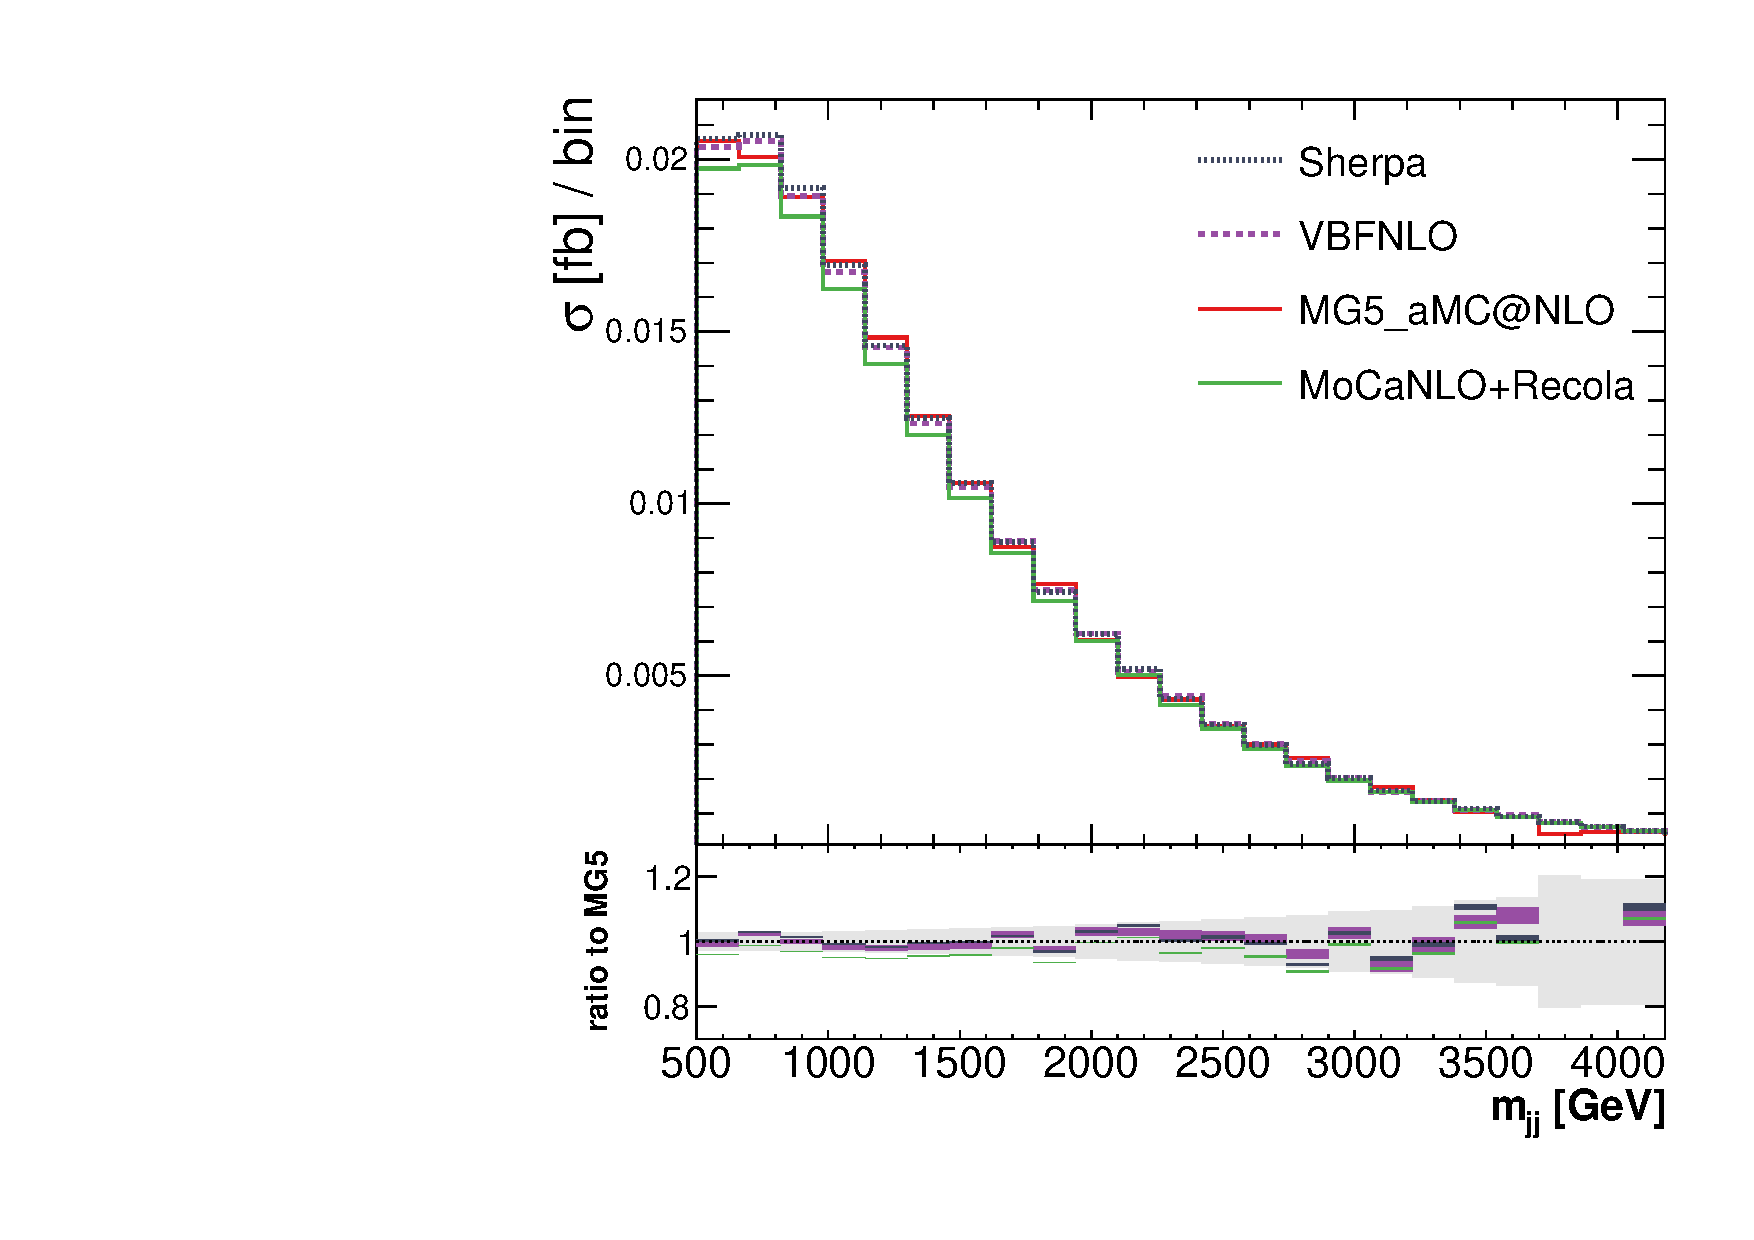
\includegraphics[scale=0.375]{figs/mjj_FixedOrder.pdf}
   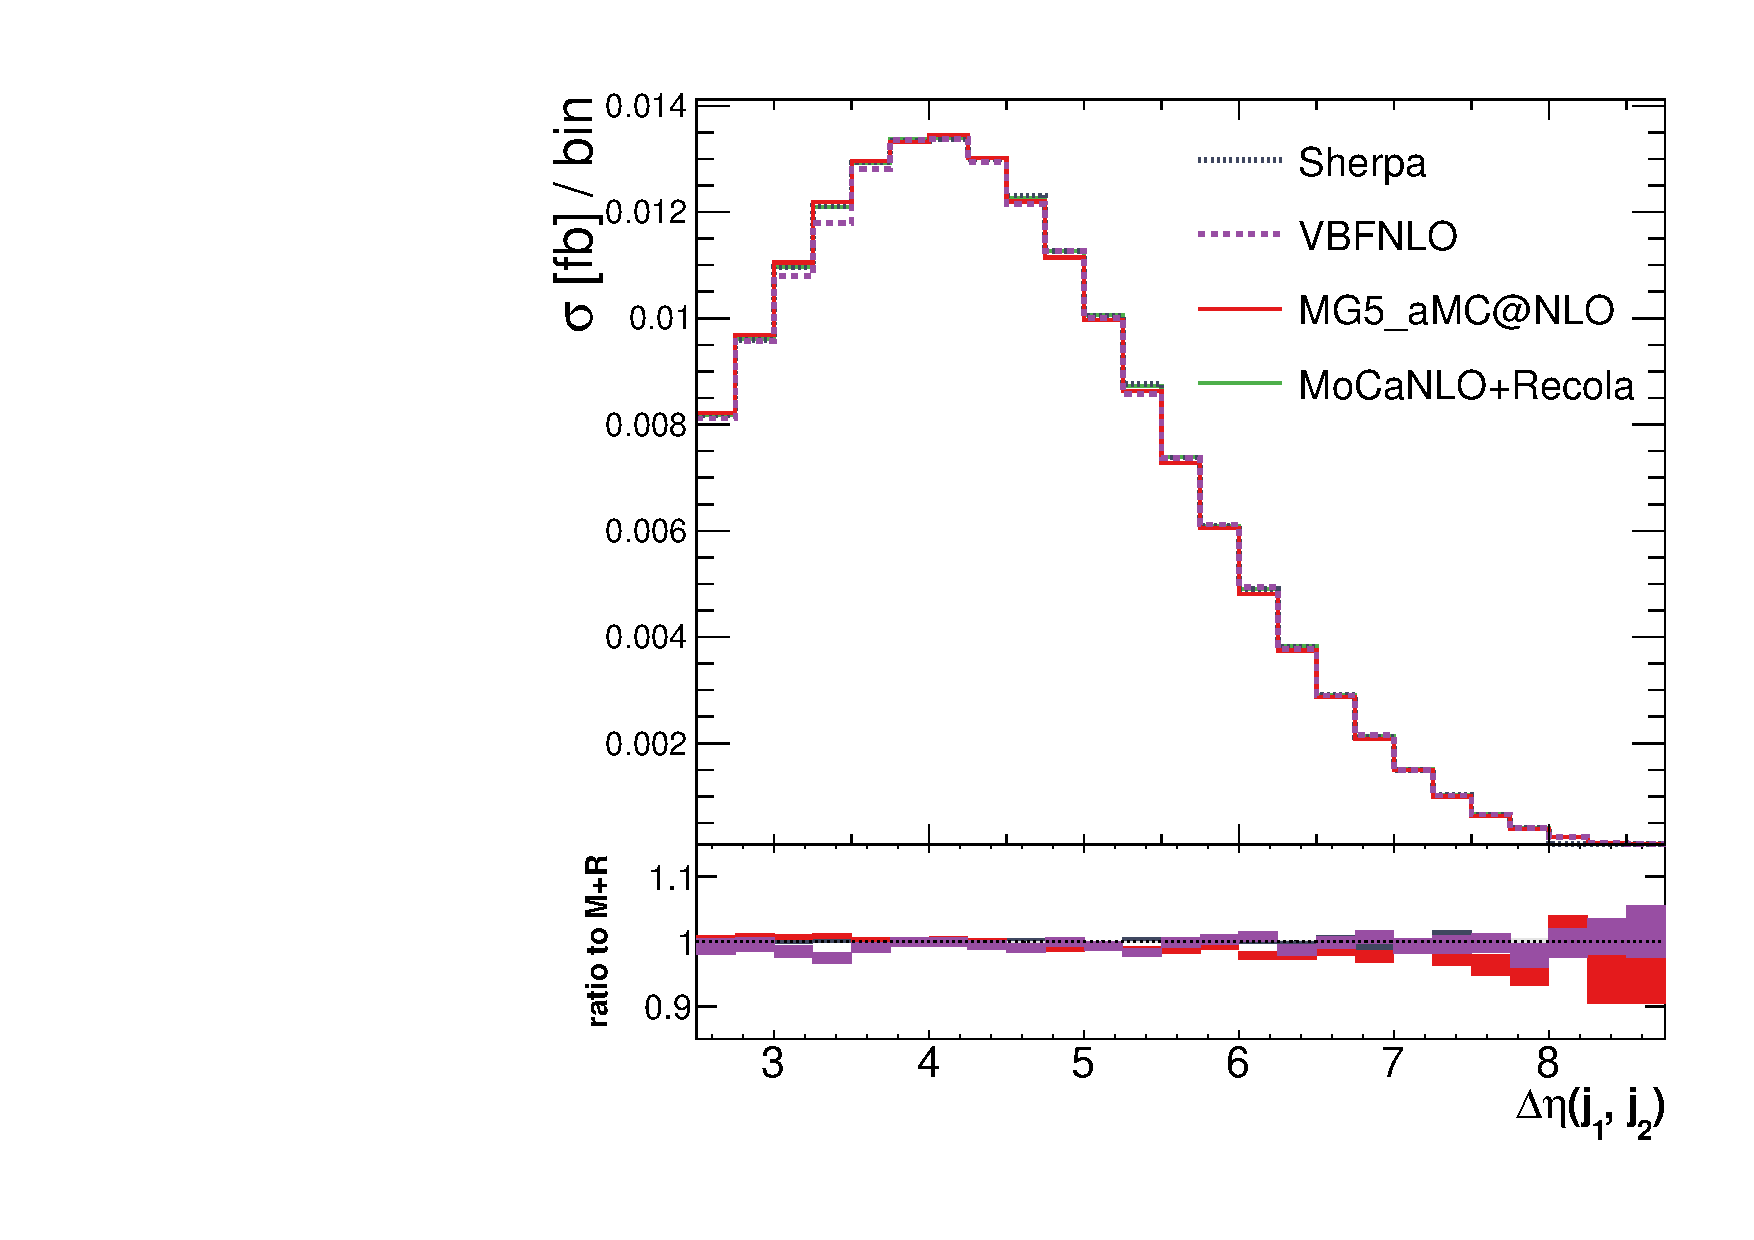
\includegraphics[scale=0.375]{figs/dEtajj_FixedOrder.pdf}
\caption{Differential distributions computed at fixed-order with centre-of-mass energy $\sqrt{s}=13{\rm~TeV}$ at the LHC for ${\rm p} {\rm p}
  \to {\rm e}^-  \nu_{\rm e}  \mu^+ \mu^- {\rm j} {\rm j}$ at LO with fixed scaled $\mu = M_{\rm W}$: 
                invariant mass of the two jets~(left),
                rapidity separation between the two jets~(right).
                The predictions in the lower plot are normalised to the ones of {\sc MG5\_aMC}. Uncertainties
                shown in the ratio plot are statistical only.
                }
\label{vbs_fig_fixed_order}
\end{center}
\end{figure}


\subsubsection*{Comparisons after parton shower}

In Figs.~\ref{vbs_fig_shower_1a} and \ref{vbs_fig_shower_1b}, a comparison of results obtained with different
generators for the process ${\rm p} {\rm p} \to {\rm e}^+  \nu_{\rm e}  \mu^+ \mu^- {\rm j} {\rm j}$ at LO supplemented with parton shower with fixed scaled $\mu =M_W$ is shown. 
In particular, in Fig.~\ref{vbs_fig_shower_1a} several differential distributions are shown:
the invariant mass of the two jets, the rapidity separation between the two jets, the transverse momentum of the anti-muon--muon system, and the distance between the two jets.
The overall picture is that the predictions obtained from {\sc Sherpa}, {\sc VBFNLO}+{\sc PYTHIA8}, and {\sc MG5\_aMC}+{\sc PYTHIA8} agree rather well over the whole kinematic range.
On the other hand, the predictions obtained from {\sc VBFNLO}+{\sc HERWIG7} seem to be very different for all type of distributions.
\MP{What is the band? Statistical error or scale uncertainty? This should be specified in the text and the caption of the plots.}
\KL{We should decide how to present the results. Since it seems something is not right with the VBFNLO+Herwig plots (they look different
    to the VBNFLO standalone + Herwig LHE showered). Do we want to show those results instead?}

\begin{figure}[htbp]
\begin{center}
   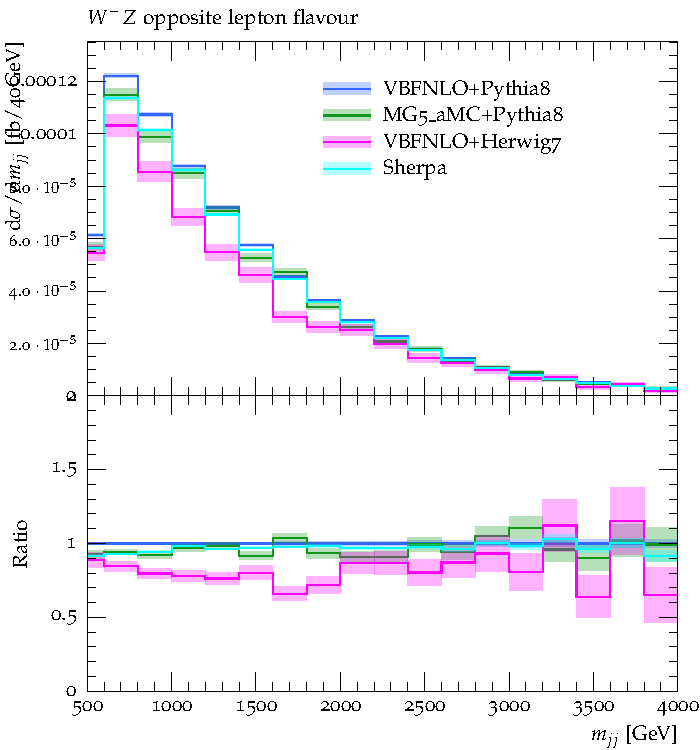
\includegraphics[scale=0.65]{figs/VBFNLO_WmZ_OF_mjj}
   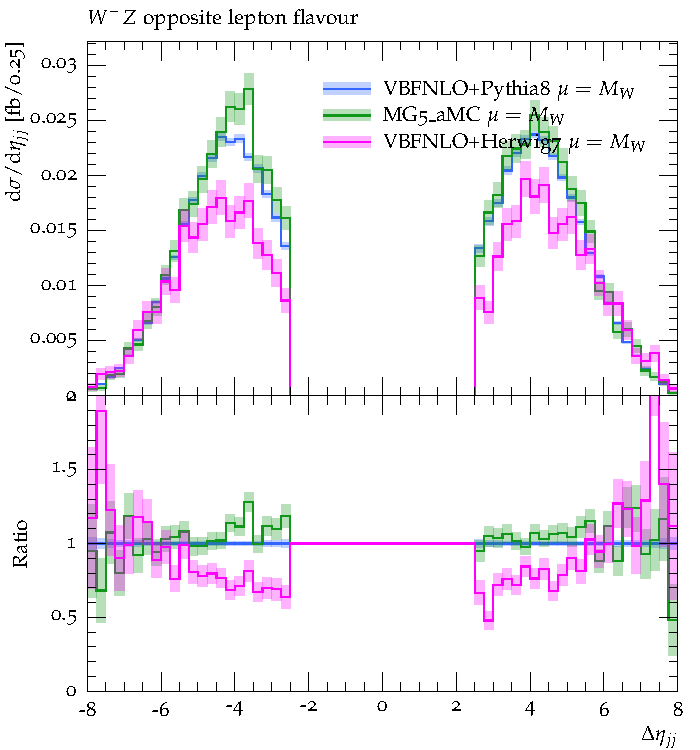
\includegraphics[scale=0.65]{figs/VBFNLO_WmZ_OF_dEtajj}
   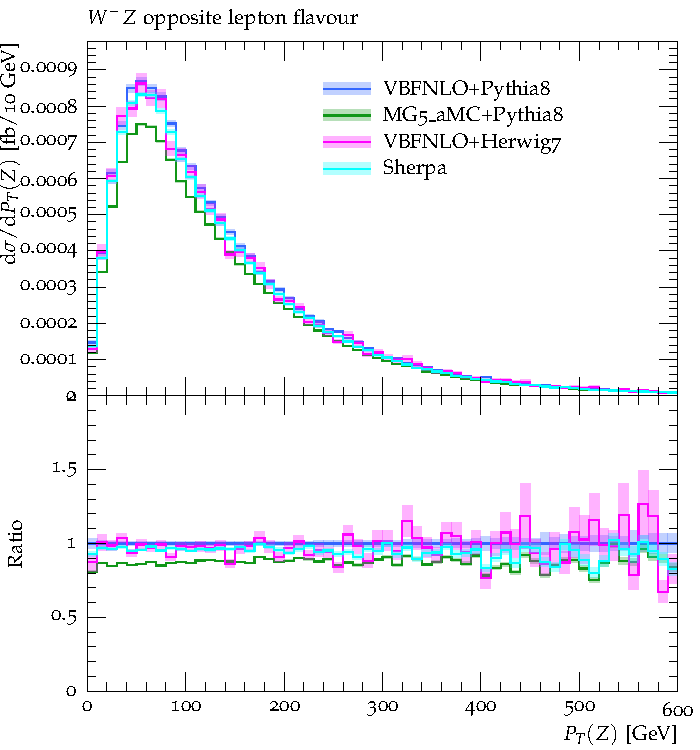
\includegraphics[scale=0.65]{figs/VBFNLO_WmZ_OF_ZPt}
   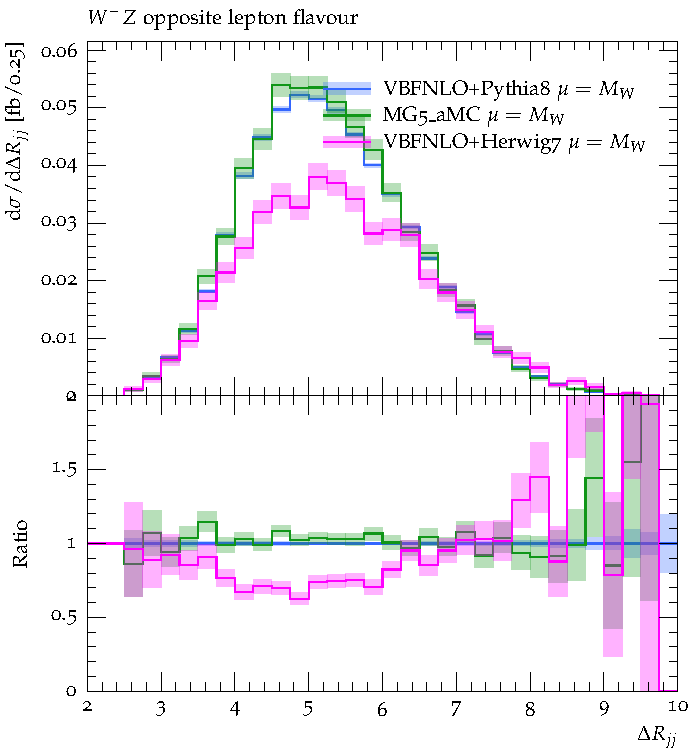
\includegraphics[scale=0.65]{figs/VBFNLO_WmZ_OF_dRjj}
\caption{Differential distributions at a centre-of-mass energy $\sqrt{s}=13{\rm TeV}$ at the LHC for ${\rm p} {\rm p}
  \to {\rm e}^-  \nu_{\rm e}  \mu^+ \mu^- {\rm j} {\rm j}$ at LO with fixed scaled $\mu = M_{\rm W}$: 
                invariant mass of the two jets~(top left),
                rapidity separation between the two jets~(top right)
                transverse momentum of the anti-muon--muon system~(bottom left), and
                distance between the two jets~(bottom right).}
\label{vbs_fig_shower_1a}
\end{center}
\end{figure}

These differences are more explicit in Fig.~\ref{vbs_fig_shower_1b}.
There, the Zeppenfeld variable for the three charged leptons and the third jet as well as the number of jets is displayed.
The Zeppenfeld variable for a given particle $X$ is defined as

\begin{equation}
  z_{X} = \frac{y_{X}-\frac{y_{{\rm j}_1}+y_{{\rm j}_2}}2}{|y_{{\rm j}_1}-y_{{\rm j}_2}|} ,
\end{equation}
%
where $y_{{\rm j}_{1/2}}$ are the rapidity of the first and second hardest jet, respectively.
The Zeppenfeld variable of the third jet, as well as the number of jets beyond two, are observables that are not defined at LO,
and are only non-zero thanks to the emissions of the parton shower.
It is thus expected that these feature an even worse agreement that the previously discussed observables, as 
significantly different algorithms are imployed by the parton shower generators we consider. 
We note that even where there are similarities, we have not taken care to tune the parameters
of the shower but rather consider the spread of predictions as reflective of the uncertainty 
of the parton shower dominated observables. While variables such as the Zeppenfeld of the third jet
have known separation power between the EW and QCD induced production, tuning an experimental selection 
on this observable would introduce large theoretical uncertainties, especially if only LO predictions
are considered. A similar argument holds for a veto on extra jet activity.

\begin{figure}[htbp]
\begin{center}
   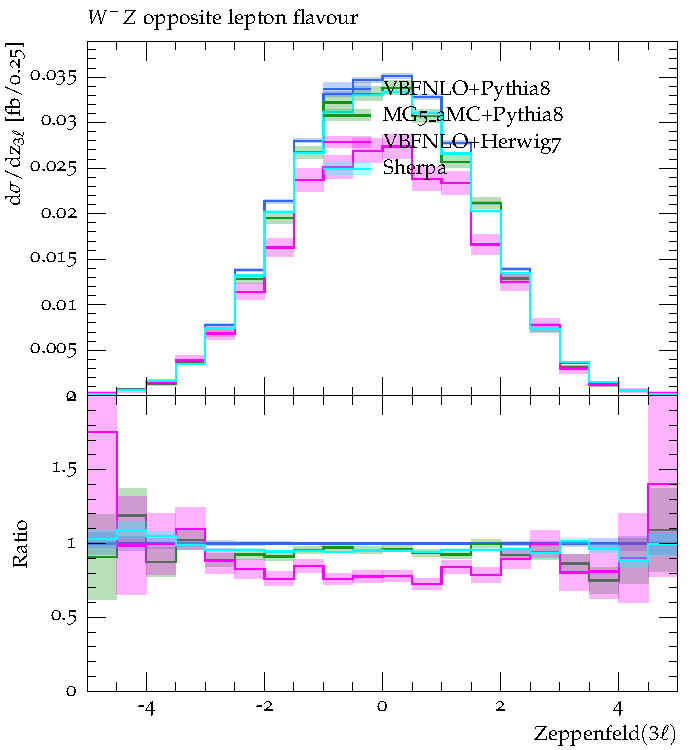
\includegraphics[scale=0.65]{figs/VBFNLO_WmZ_OF_zep3l}
   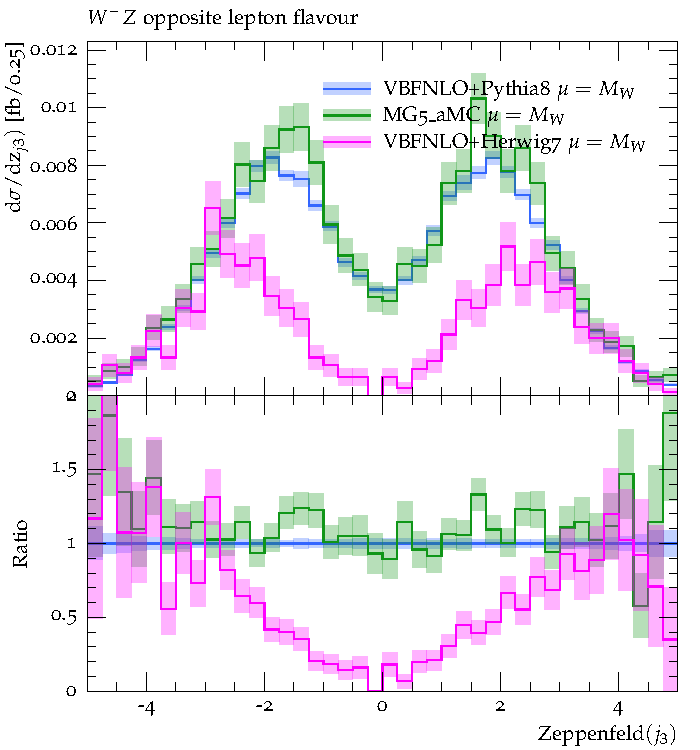
\includegraphics[scale=0.65]{figs/VBFNLO_WmZ_OF_zepj3}
   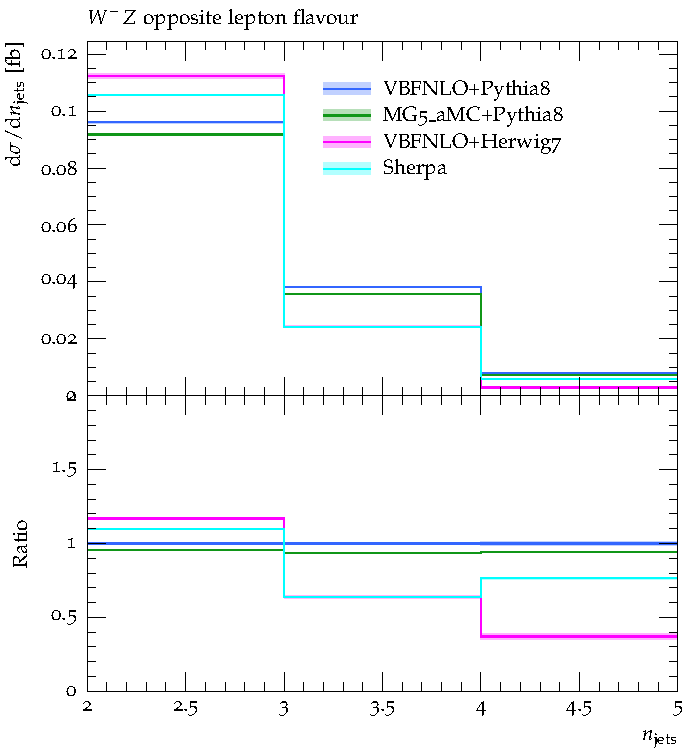
\includegraphics[scale=0.65]{figs/VBFNLO_WmZ_OF_nJets}
\caption{Differential distributions at a centre-of-mass energy $\sqrt{s}=13{\rm TeV}$ at the LHC for ${\rm p} {\rm p}
  \to {\rm e}^-  \nu_{\rm e}  \mu^+ \mu^- {\rm j} {\rm j}$ at LO with fixed scaled $\mu = M_{\rm W}$: 
                Zeppenfeld variable for the three leptons~(top left),
                Zeppenfeld variable for the third jet~(top right)
                number of jets~(bottom).
                \MP{Range of the number of jets not correct.}}
\label{vbs_fig_shower_1b}
\end{center}
\end{figure}

In Figs.~\ref{vbs_fig_shower_2a} and \ref{vbs_fig_shower_2b} results are compared between fixed scale $\mu = M_{\rm W}$ and dynamic scale $\mu = {\rm Max}\left[p_{\rm T, j}\right]$.
In particular, predictions for {\sc Sherpa} and {\sc MG5\_aMC} for both scales are presented.
The observables displayed are the same as for the previous comparison.
For the invariant mass of the two jets as well as the transverse momentum of the anti-muon--muon system, we see that for both generators, the use of fixed scale enhance the predictions toward high transverse momentum.
For the rapidity separation of the two jets as well as the distance between the two jets, the shape difference between fixed and dynamical scale is not present for {\sc MG5\_aMC}.
On the other hand, in {\sc Sherpa}, the use of fixed scale enhance the predictions for small separations.

\begin{figure}[htbp]
\begin{center}
   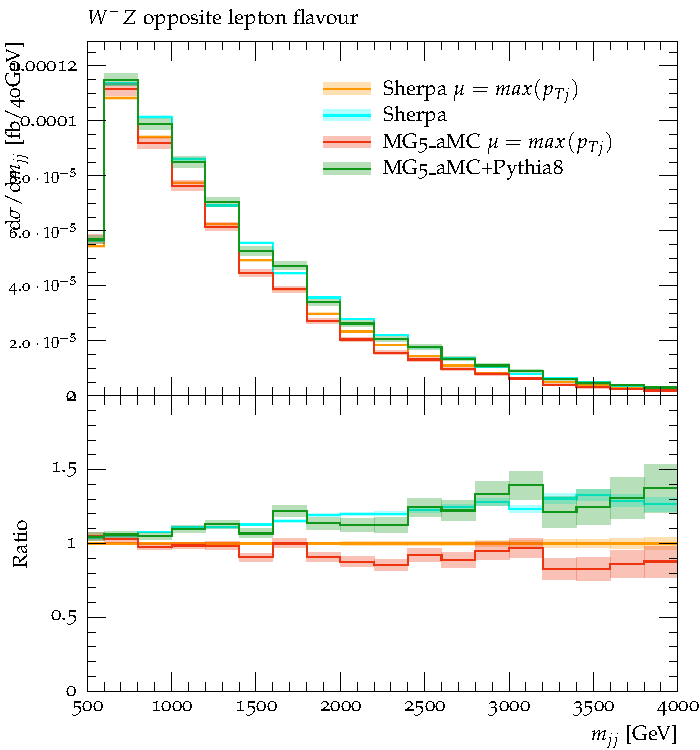
\includegraphics[scale=0.65]{figs/dyn_WmZ_OF_mjj}
   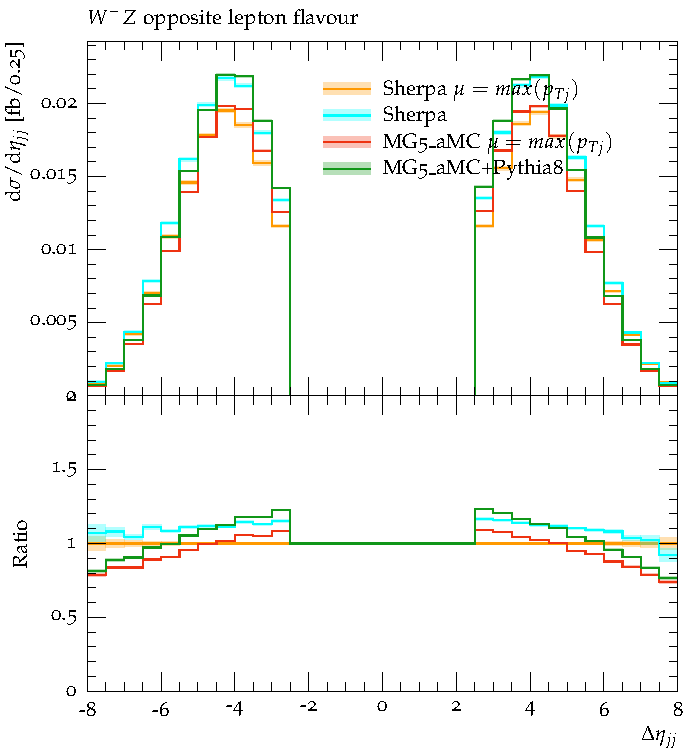
\includegraphics[scale=0.65]{figs/dyn_WmZ_OF_dEtajj}
   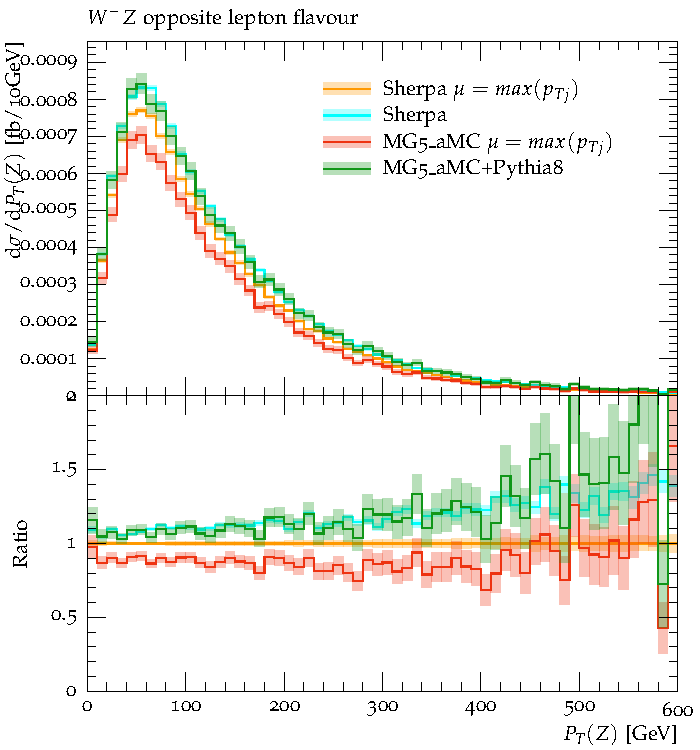
\includegraphics[scale=0.65]{figs/dyn_WmZ_OF_ZPt}
   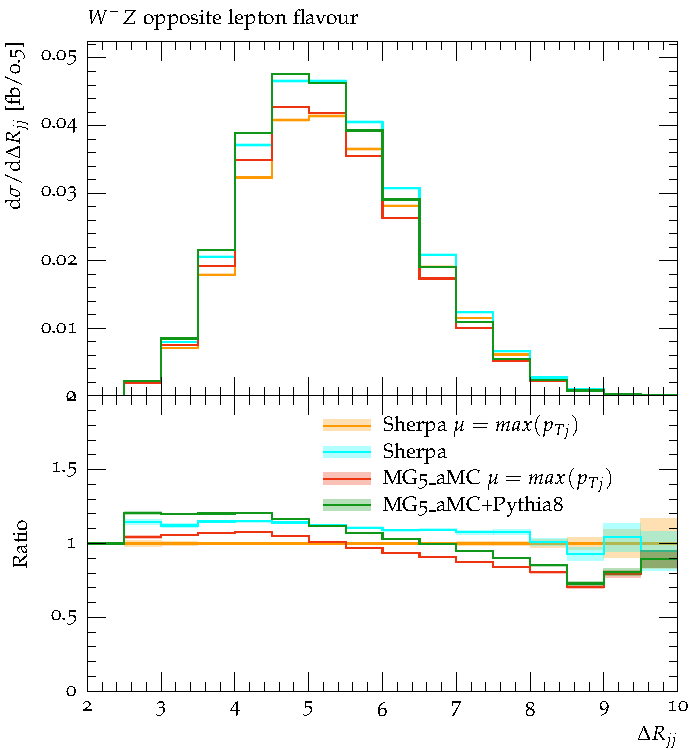
\includegraphics[scale=0.65]{figs/dyn_WmZ_OF_dRjj}
\caption{Differential distributions at a centre-of-mass energy $\sqrt{s}=13{\rm TeV}$ at the LHC for ${\rm p} {\rm p}
  \to {\rm e}^-  \nu_{\rm e}  \mu^+ \mu^- {\rm j} {\rm j}$ at LO with fixed and dynamic scale values:  
                invariant mass of the two jets~(top left),
                rapidity separation between the two jets~(top right)
                transverse momentum of the anti-muon--muon system~(bottom left), and
                distance between the two jets~(bottom right).
                In the lower plots, the predictions are normalised to the ones of {\sc Sherpa} with dynamical scale.}
\label{vbs_fig_shower_2a}
\end{center}
\end{figure}

Concerning the last set of observables (Zeppenfeld variable of the three leptons and third jet as well as the number of jets) in Fig.~\ref{vbs_fig_shower_2b}, the use of fixed or dynamical scale does not seem to have a large impact.
The only clearly visible differences between fixed and dynamical scale is the normalisation.
This effect was already observed at the level of the fiducial cross section in Tables~\ref{table:xsectLOfix} and \ref{table:xsectLOdyn}.
There the effect of the different scale amount to a change in normalisation of about $12\%$ for both ${\rm p}{\rm p}\to{\rm e}^+\nu_{\rm e}\mu^+\mu^-{\rm j}{\rm j}$ and ${\rm p}{\rm p}\to{\rm e}^-\bar\nu_{\rm e}\mu^+\mu^-{\rm j}{\rm j}$ processes.

\begin{figure}[htbp]
\begin{center}
   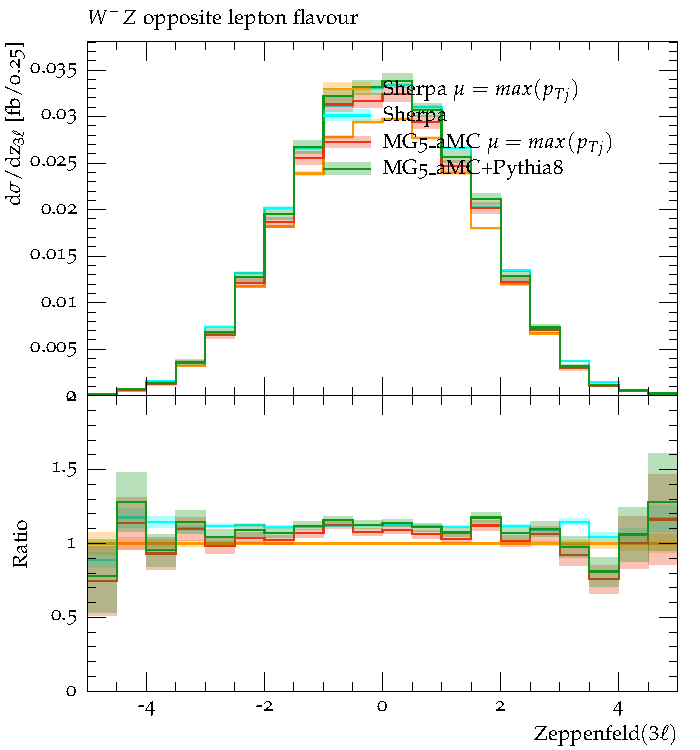
\includegraphics[scale=0.65]{figs/dyn_WmZ_OF_zep3l}
   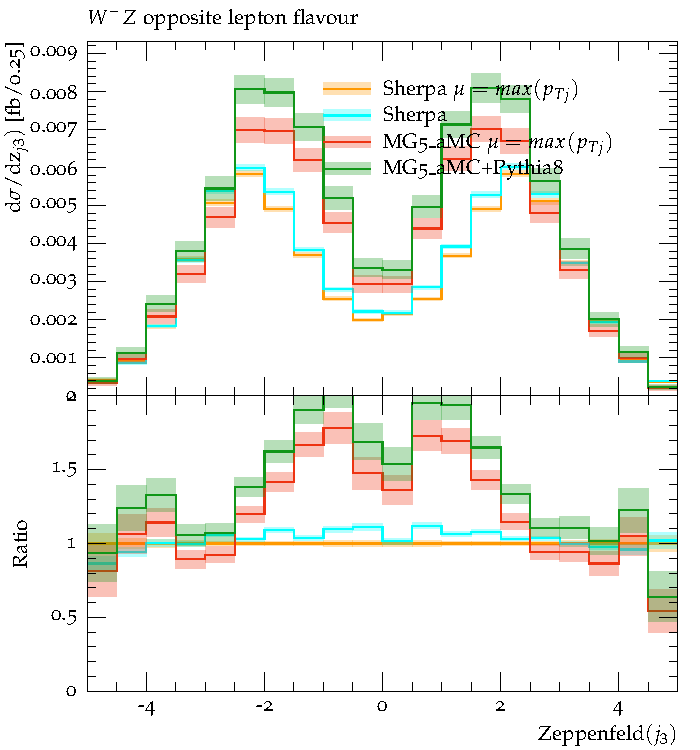
\includegraphics[scale=0.65]{figs/dyn_WmZ_OF_zepj3}
   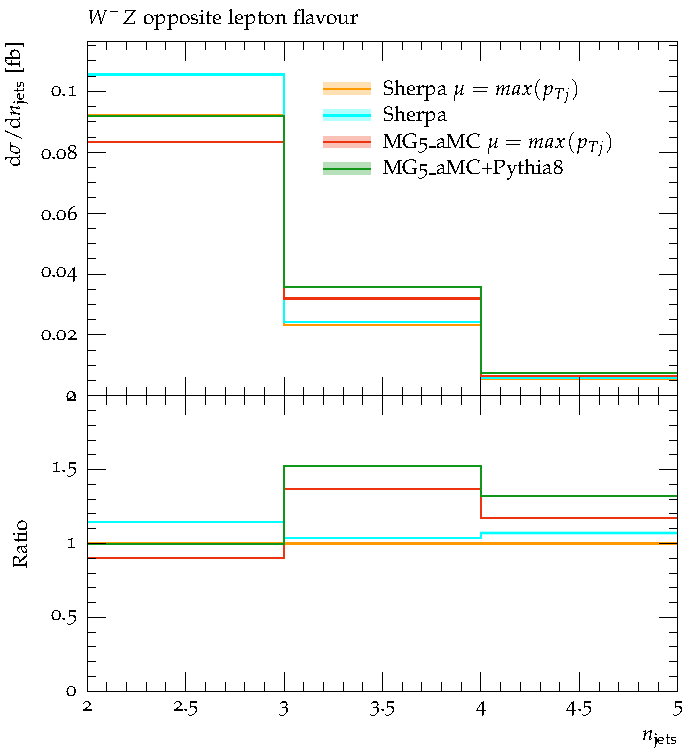
\includegraphics[scale=0.65]{figs/dyn_WmZ_OF_nJets}
\caption{Differential distributions at a centre-of-mass energy $\sqrt{s}=13{\rm TeV}$ at the LHC for ${\rm p} {\rm p} \to {\rm e}^-  \nu_{\rm e}  \mu^+ \mu^- {\rm j} {\rm j}$ at LO with fixed and dynamic scale values: 
                Zeppenfeld variable for the three leptons~(top left),
                Zeppenfeld variable for the third jet~(top right)
                number of jets~(bottom).
                In the lower plots, the predictions are normalised to the ones of {\sc Sherpa} with dynamical scale.
                \MP{Range of the number of jets not correct.}
                }
\label{vbs_fig_shower_2b}
\end{center}
\end{figure}

